\chapter{Diseño e implementación}
\label{cap:DisenioImplementacion}

En este capítulo se presenta la arquitectura de hardware y software del dispositivo de captura, como así también del generador de señal MVB desarrollado para probar el dispositivo de captura sin necesidad de conectarlo en una formación ferroviaria.

\section{Arquitectura de hardware}
\label{sec:hardware}

Como se muestra en la figura~\ref{fig:conexion}, el dispositivo de captura tiene dos conectores DE-9 compatibles con el medio EMD. De esta manera se lo puede conectar a un segmento MVB entre dos dispositivos cualesquiera.

\begin{figure}[htbp]
	\centering
    {
        \fontfamily{phv}
        \fontsize{8pt}{8pt}\selectfont
        \input{./Figures/conexion.pdf_tex}
    }
	\caption{Conexión del dispositivo de captura en un segmento EMD.}
    \label{fig:conexion}
\end{figure}

En la figura~\ref{fig:bloques} se muestra un diagrama de la arquitectura del dispositivo de captura.
Se dejan en corto circuito las líneas de transmisión (ver figura~\ref{fig:pines}), de forma tal de que el dispositivo opere en forma pasiva. Salvando la impedancia que agrega a la línea, el dispositivo de captura es transparente para el resto de los dispositivos del segmento.
El dispositivo MAX485 \cite{max485} se utiliza para convertir la señal de entrada (par diferencial $-$5~V - +5~V) a una señal compatible para el analizador lógico VKTECH (0~V - +5~V). El analizador lógico se conecta a una Raspberry Pi mediante un puerto USB 2.0. La Raspberry Pi decodifica las tramas por software y almacena los datos capturados en una tarjeta de memoria. Mediante su interfaz Wi-Fi se puede conectar una PC (utilizando el protocolo SSH) para descargar las capturas, y también para visualizar el tráfico del bus MVB en tiempo real.

\begin{figure}[htbp]
	\centering
    {
        \fontfamily{phv}
        \fontsize{8pt}{8pt}\selectfont
        \input{./Figures/bloques.pdf_tex}
    }
	\caption{Arquitectura de hardware del dispositivo de captura.}
    \label{fig:bloques}
\end{figure}

En la figura~\ref{fig:esquematico} se muestra un diagrama esquemático con el detalle de las conexiones entre los diferentes componentes. En el diagrama se utiliza la etiqueta ``USB'' para representar la conexión a la Raspberry Pi, que no se muestra por simplicidad. Asimismo, la conexión ``VCC'' del MAX485 se conecta al pin número 2 del conector GPIO de la Raspberry Pi \cite{gpio}.

\begin{figure}[htbp]
	\centering
	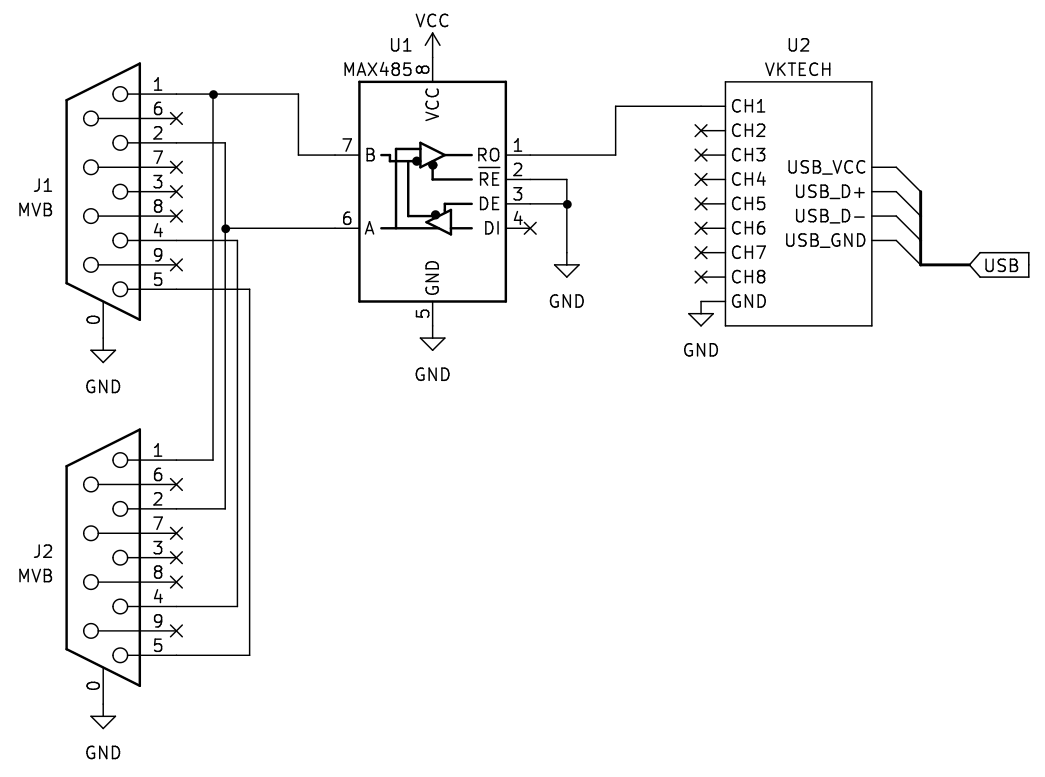
\includegraphics[width=1\textwidth]{./Figures/esquematico.png}
	\caption{Diagrama esquemático del dispositivo de captura.}
    \label{fig:esquematico}
\end{figure}

En la figura~\ref{fig:fotodispositivo} se muestra una foto del dispositivo de captura en construcción. Cabe aclarar que en el dispositivo hay cuatro MAX485 para permitir, en el futuro, capturar ambas líneas A y B del segmento EMD, o bien capturar dos o más segmentos diferentes. En esta primera versión del dispositivo se utiliza solo uno de los MAX485.

\begin{figure}[htbp]
	\centering
	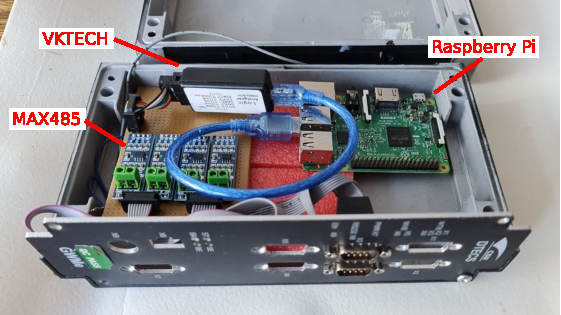
\includegraphics[width=1\textwidth]{./Figures/foto-dispositivo.pdf}
	\caption{Foto del dispositivo de captura en construcción.}
    \label{fig:fotodispositivo}
\end{figure}

\section{Arquitectura de software}
\label{sec:software}

Como se ve en la figura~\ref{fig:bloques}, la señal digital capturada por el VKTECH se envía a la Raspberry Pi en tiempo real mediante la interfaz USB. Para recibir esta señal en la Raspberry Pi se utiliza Sigrok, invocándolo de la siguiente manera:

\begin{lstlisting}[basicstyle=\small,breaklines=true]
$ sigrok-cli -d fx2lafw --continuous --config samplerate=12m
             --channels D0 -O binary
\end{lstlisting}

Los parámetros utilizados son:

\begin{itemize}
    \item \texttt{-d fx2lafw}: utilizar el \textit{driver} compatible con el dispositivo VKTECH.
    \item \texttt{--continuous}: muestrear en forma continua hasta ser detenido.
    \item \texttt{--config samplerate=12m}: muestrear con una frecuencia de 12 MHz.
    \item \texttt{--channels D0}: muestrear únicamente el canal 0 (correspondiente al pin \texttt{CH1} de la figura \ref{fig:esquematico}).
    \item \texttt{-O binary}: producir como salida un flujo de datos en formato binario.
\end{itemize}

Por cada muestra capturada, se emite un byte en el que cada bit corresponde a uno de los 8 canales del VKTECH.
Como se captura únicamente el canal 0, el bit menos significativo será 0 o 1 dependiendo de si la señal lógica capturada es baja o alta.
De esta forma, el flujo de datos tiene un ancho de banda de 12 MB/s, aunque se usa solo uno de los 8 bits de cada byte.
Este flujo de datos se puede redireccionar a un archivo o a un \textit{pipe} de Unix.

En la figura~\ref{fig:sigrok} se muestra un ejemplo del flujo de datos producido por Sigrok. El intervalo de 666,7 ns corresponde a un bit de datos de una trama MVB en codificación Manchester (ver figura~\ref{fig:manchester}). La frecuencia de muestreo de 12 MHz produce una muestra cada 83,33 ns.

\begin{figure}[htbp]
	\centering
    {
        \fontfamily{phv}
        \fontsize{9pt}{9pt}\selectfont
        \input{./Figures/sigrok.pdf_tex}
    }
	\caption{Flujo de datos producido por Sigrok.}
    \label{fig:sigrok}
\end{figure}

Sería posible bajar la frecuencia de muestreo, pero dado que la señal MVB se transmite a 1,5 Mbit/s en codificación Manchester, para lograr una captura suficientemente confiable el límite inferior es 6 MHz.
Sin embargo, la captura en una frecuencia cercana al límite inferior aumenta considerablemente la tasa de errores de captura.
La frecuencia elegida de 12 MHz ofrece un buen balance entre confiabilidad y eficiencia en espacio.

El flujo de datos producido por Sigrok se redirecciona mediante un \textit{pipe} de Unix a un software programado en lenguaje Go. Como se muestra en la figura~\ref{fig:capas-software}, la decodificación se realiza en tres capas de procesamiento:

\begin{enumerate}
\item La capa inferior (\texttt{MVBStream}) lee el flujo de datos byte por byte y ofrece funcionalidades tales como leer muestras individualmente, esperar hasta la siguiente transición de estado (alto-bajo o bajo-alto), esperar una cantidad de tiempo, etc.
\item La capa intermedia (\texttt{MVBDecoder}) identifica las tramas MVB y por cada telegrama produce un evento (\texttt{Event}).
\item La capa superior recibe los eventos y los procesa según el modo de operación del software. Se ofrecen dos modos de operación:
    \begin{itemize}
        \item En el modo interactivo, el software presenta una interfaz de usuario en la que se muestra el tráfico MVB en tiempo real.
        \item En el modo de almacenamiento, el software permite almacenar la evolución histórica de una o más variables de importancia.
    \end{itemize}
\end{enumerate}

\begin{figure}[htbp]
	\centering
    {
        \fontfamily{phv}
        \fontsize{9pt}{9pt}\selectfont
        \input{./Figures/capas-software.pdf_tex}
    }
	\caption{Capas de procesamiento del software de captura.}
    \label{fig:capas-software}
\end{figure}

En la figura~\ref{fig:interactivo} se muestra una captura de pantalla del modo interactivo.
En esta pantalla se presenta al usuario un resumen de la información capturada en tiempo real.
En la figura se destacan algunas secciones de la pantalla, que se detallan a continuación.

\begin{enumerate}
\item Total de telegramas capturados desde el inicio.
\item Cantidad de tiempo transcurrido desde el inicio.
\item Histograma de la cantidad de telegramas capturados en los últimos 10 segundos.
\item Tasa de telegramas capturados por segundo.
\item Histograma y tasa de telegramas por segundo, desglosado por el valor del \texttt{F\_code}.
\item Listado del último valor transmitido de cada variable, ordenado por puerto. El usuario puede elegir el rango de puertos a visualizar en esta lista.
\item Histograma y listado de los últimos errores de decodificación.
\end{enumerate}

\begin{figure}[htbp]
	\centering
	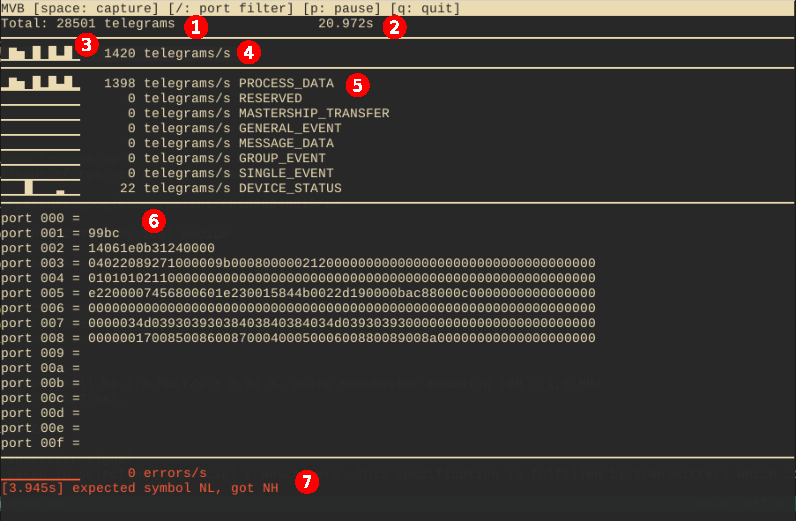
\includegraphics[width=1\textwidth]{./Figures/modo-interactivo.pdf}
	\caption{Modo interactivo del software de captura.}
    \label{fig:interactivo}
\end{figure}

En el modo de almacenamiento, el software se configura con un conjunto de variables a capturar, y almacena la evolución histórica de dichas variables.
Para el almacenamiento histórico se genera una carpeta por cada día de captura, y en cada carpeta un archivo CSV por cada variable capturada.

Por ejemplo, si se desea capturar los primeros 6 bytes del puerto \texttt{0x002} y el byte 8 del puerto \texttt{0x003}, se debe ejecutar el programa de la siguiente manera:

\begin{lstlisting}[basicstyle=\small,breaklines=true]
$ go run record/main.go 002:0:6 "fecha y hora" 003:8:9 "tension de red"
\end{lstlisting}

En la figura~\ref{fig:carpetas} se muestra la estructura de carpetas y archivos generada por el software al ser ejecutado con esta configuración.
Cada línea de los archivos CSV tiene el formato \texttt{<hora>,\allowbreak <valor>}, donde \texttt{<hora>} es la hora exacta en la que se transmitió la variable y \texttt{<valor>} es el valor de la variable.
Para conservar espacio, solo se agrega una línea al archivo CSV cuando la variable cambia de valor.

\begin{figure}[htbp]
	\centering
    {
        \ttfamily
        \fontsize{8pt}{8pt}\selectfont
        \input{./Figures/carpetas.pdf_tex}
    }
	\caption{Ejemplo de estructura de carpetas y archivos generado por el software en modo de almacenamiento.}
    \label{fig:carpetas}
\end{figure}

El código fuente de este programa está disponible en la plataforma Github \cite{mvbparse-go}.
En el archivo \texttt{README.md} se muestran más detalles acerca de los diferentes modos de funcionamiento.

\section{Generador de señal de prueba MVB}
\label{sec:generador}

Para probar el funcionamiento del software de captura sin necesidad de acudir a un taller de Trenes Argentinos y conectar el dispositivo en una formación ferroviaria, se decidió desarrollar un dispositivo auxiliar. Este dispositivo genera una señal con características similares a la señal transmitida en el bus MVB, emitiendo una secuencia de tramas en forma cíclica.

En la figura~\ref{fig:generador} se muestra un diagrama de bloques con el generador de señal MVB conectado al VKTECH. La señal es generada por software en una EDU-CIAA, y se transmite mediante la interfaz SPI. La señal generada es similar a la señal producida por el MAX485 en la figura~\ref{fig:bloques}.

\begin{figure}[htbp]
	\centering
    {
        \fontfamily{phv}
        \fontsize{8pt}{8pt}\selectfont
        \input{./Figures/generador.pdf_tex}
    }
	\caption{Generador de señal MVB.}
    \label{fig:generador}
\end{figure}

El firmware desarrollado para el generador de señal está disponible en la plataforma Github \cite{mvbgen}.

Para simular el tráfico del bus, el firmware transmite un telegrama cada 750 microsegundos.
Los telegramas transmitidos son reproducciones de capturas realizadas en un bus MVB real (ver sección \ref{sec:capturas}). Por ejemplo, en el código~\ref{cod:telegrama} se muestra la definición del primer telegrama transmitido.
Los primeros 3 bytes corresponden a la trama \textit{master} (16 bits de datos más la secuencia de verificación) y a continuación se especifica el contenido de la trama \textit{slave}, de 36 bytes de longitud.

\begin{lstlisting}[label=cod:telegrama,caption=Definición de un telegrama a transmitir (\texttt{gen.c}).,float,numberstyle=\footnotesize\ttfamily,language=C,breaklines=true,numbers=left,firstnumber=11,xleftmargin=1cm]
static const telegram_t mvb_data[] = {
    { { 0x43, 0x90, 0xd6 }, (uint8_t[]){ 0x97, 0x1e, 0x00, 0x00, 0x00, 0x82, 0x14, 0x06, 0xdf, 0x1e, 0x0b, 0x31, 0x0f, 0x00, 0x17, 0x05, 0x8c, 0xf8, 0x00, 0x00, 0x00, 0x00, 0x00, 0x00, 0x03, 0x4d, 0xc9, 0x11, 0x94, 0x11, 0xa8, 0x11, 0xa8, 0x04, 0x05, 0x88 }, 36 },
\end{lstlisting}

Para enviar un telegrama, se envía la trama \textit{master}, luego se transmiten 15 bits en alto (esto simula una pequeña pausa entre las tramas), y luego se transmite la trama \textit{slave}. Esta secuencia de pasos se muestra en el código~\ref{cod:send}.

\begin{lstlisting}[label=cod:send,caption=Secuencia de pasos para transmitir un telegrama (\texttt{gen.c}).,float,numberstyle=\footnotesize\ttfamily,language=C,breaklines=true,numbers=left,firstnumber=193,xleftmargin=1cm]
    send_master(mvb_data[i].master);
    send_idle(15, 1);
    send_slave(mvb_data[i].slave, mvb_data[i].slave_len);
\end{lstlisting}

Como se muestra en el código~\ref{cod:sendmaster}, para transmitir la trama \textit{master}, se envía el delimitador inicial, seguido de los 3 bytes de la trama y el delimitador final. La transmisión de la trama \textit{slave} es similar.

\begin{lstlisting}[label=cod:sendmaster,caption=Secuencia de pasos para transmitir la trama \textit{master} (\texttt{gen.c}).,float,numberstyle=\footnotesize\ttfamily,language=C,breaklines=true,numbers=left,firstnumber=173,xleftmargin=1cm]
static void send_master(const uint8_t bytes[]) {
    send_start_bit();
    send_master_start_delimiter();
    send_bytes(bytes, 3);
    send_end_delimiter();
}
\end{lstlisting}

Las funciones previamente mencionadas cargan la información a transmitir en un \textit{buffer}. Cada bit de información se codifica en Manchester: un bit ``1'' corresponde a una transición negativa y se traduce en dos bits 1-0, y un bit ``0'' corresponde a una transición positiva y se traduce en dos bits 0-1. De esta manera, cada bit de información que se carga ocupa 2 bits en el \textit{buffer}.

En el código~\ref{cod:main} se muestra el ciclo principal del programa, en el que se hace una pausa de 750 microsegundos, luego se prepara el siguiente telegrama a transmitir en el \textit{buffer}, y luego se transmite el contenido del \textit{buffer} mediante la interfaz SPI.

\begin{lstlisting}[label=cod:main,caption=Ciclo principal del programa (\texttt{main.c}).,float,numberstyle=\footnotesize\ttfamily,language=C,breaklines=true,numbers=left,firstnumber=31,xleftmargin=1cm]
    while (1) {
        delayInaccurateUs(750);
        sendbuf_t *buf = next_telegram();
        spiWrite(SPI0, buf->data, buf->bytes);
    }
\end{lstlisting}

La interfaz SPI se configura para transmitir con una frecuencia de 3 Mbit/s, de forma tal que cada par de bits transmitidos corresponden a un bit de información codificada en Manchester. De esta manera se logra una tasa de 1,5 Mbit/s compatible con el protocolo MVB.
